%%%%%%%%%%%%%%%%%%%%%%%%%%%%%%%%%%%%%%%%%%%%%%%%%%%%%%%%%%%%%%%%%%%%%%%%%%%
%% This file is part of the book
%%
%% Algorithmic Graph Theory
%% http://code.google.com/p/graph-theory-algorithms-book/
%%
%% Copyright (C) 2009, 2010 Minh Van Nguyen <nguyenminh2@gmail.com>
%%
%% See the file COPYING for copying conditions.
%%%%%%%%%%%%%%%%%%%%%%%%%%%%%%%%%%%%%%%%%%%%%%%%%%%%%%%%%%%%%%%%%%%%%%%%%%%

%% simple graph
\subfigure[Simple graph.]{
\label{fig:introduction:triangle_simple_graph}
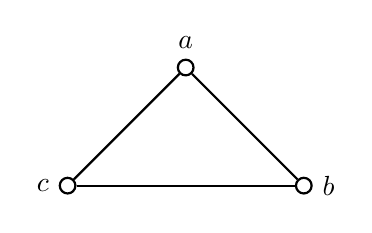
\begin{tikzpicture}
[nodedecorate/.style={shape=circle,inner sep=2pt,draw,thick},%
  linedecorate/.style={-,thick}]
%% nodes or vertices
\foreach \nodename/\x/\y/\direction/\navigate in {c/-1.5/0/left/west,
  b/1.5/0/right/east, a/0/1.5/above/north}
{
  \node (\nodename) at (\x,\y) [nodedecorate] {};
  \node [\direction] at (\nodename.\navigate) {$\nodename$};
}
%% edges or lines
\path
\foreach \startnode/\endnode in {a/b, b/c, c/a} {
  (\startnode) edge[linedecorate] node {} (\endnode)
};
\end{tikzpicture}
}
\quad
%%
%% digraph
\subfigure[Digraph.]{
\label{fig:introduction:triangle_digraph}
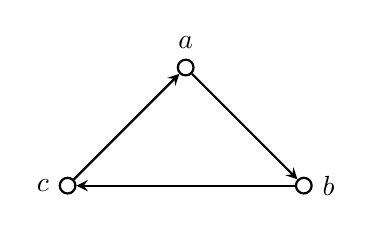
\begin{tikzpicture}
[nodedecorate/.style={shape=circle,inner sep=2pt,draw,thick},%
  arrowdecorate/.style={->,>=stealth,thick}]
%% nodes or vertices
\foreach \nodename/\x/\y/\direction/\navigate in {c/-1.5/0/left/west,
  b/1.5/0/right/east, a/0/1.5/above/north} {
  \node (\nodename) at (\x,\y) [nodedecorate] {};
  \node [\direction] at (\nodename.\navigate) {$\nodename$};
}
%% edges or lines
\path
\foreach \startnode/\endnode in {a/b, b/c, c/a} {
  (\startnode) edge[arrowdecorate] node {} (\endnode)
};
\end{tikzpicture}
}
\quad
%%
%% multidigraph
\subfigure[Multidigraph.]{
\label{fig:introduction:Konigsberg_multidigraph}
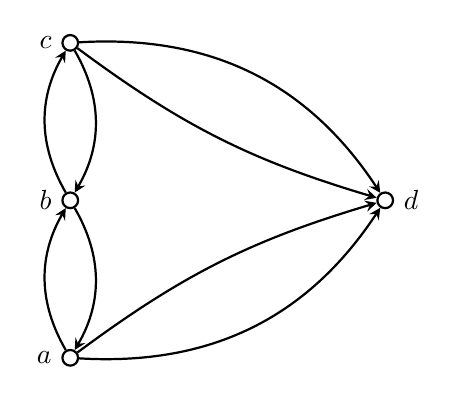
\begin{tikzpicture}
[nodedecorate/.style={shape=circle,inner sep=2pt,draw,thick},%
  arrowdecorate/.style={->,>=stealth,thick}]
%% nodes or vertices
\foreach \nodename/\x/\y in {a/0/0, b/0/2, c/0/4, d/4/2} {
  \node (\nodename) at (\x,\y) [nodedecorate] {};
}
\foreach \nodename/\direction/\navigate in {a/left/west, b/left/west,
  c/left/west} {
  \node [\direction] at (\nodename.\navigate) {$\nodename$};
}
\node [right] at (d.east) {$d$};
%% edges or lines
\path
\foreach \startnode/\endnode in {a/b, b/c} {
  (\startnode) edge[arrowdecorate,bend left] node {} (\endnode)
};
\path
\foreach \startnode/\endnode in {c/b, b/a} {
  (\startnode) edge[arrowdecorate,bend left] node {} (\endnode)
};
%% multiple directed edges
\path
(a) edge[arrowdecorate,bend left=10] node {} (d)
(c) edge[arrowdecorate,bend left] node {} (d)
(a) edge[arrowdecorate,bend right] node {} (d)
(c) edge[arrowdecorate,bend right=10] node {} (d);
\end{tikzpicture}
}
